\scanpage{41}
\deleted{
\[
\begin{array}{ccc}\mathcal X_0&\mathcal X_1&\mathcal X_2\\ \shortparallel&\shortparallel&\shortparallel\\ S&A&F\end{array}
\]
\[
\begin{aligned}
&x_0\!-\!\unsure{x_{p-1}}\ x_p\ \underbrace{x_{p+1}}\ \cdots\ x_{n-1}\ x_n\\
&\hspace{4em}\diagup\,y_1\!-\!y_2\ \cdots\ y_n\\
&\hspace{2em}x_0\!-\!x_1\!-\!x_2\ \cdots\!-\!x_n
\end{aligned}
\]
\figure{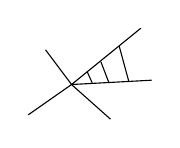
\begin{tikzpicture}[scale=.55]
\draw (-1,-.7)--(0,0)--(.9,-.8) (0,0)--(-.6,.8) (0,0)--(1.6,1.3) (0,0)--(1.85,.1);
\draw (.48,.03)--(.36,.3) (.86,.05)--(.68,.52) (1.32,.08)--(1.1,.89);
\end{tikzpicture}}

\diagram{\begin{tikzcd}[ampersand replacement=\&,row sep=tiny,column sep=tiny]
\&\&\bullet\arrow[dl]\&\bullet\arrow[l]\arrow[d]\\
\&\bullet\&\&\bullet\arrow[ll]\\
\bullet\arrow[ur]\&\&\bullet\arrow[ul]\&\\
\&\bullet\arrow[ul]\arrow[ur]\&\&
\end{tikzcd}}

a) $\forall f\in F$, les $s\in S$ et $a\in A$ incidents \unsure{à|:} $f$ forment un polygône, donc

a) Si $a<f$ ($a\in A$) $a$ a \unsure{exact\textsuperscript{t}} 2 sommets

\figure{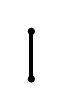
\begin{tikzpicture}[scale=.55]\draw[line width=1.4pt](0,0)--(0,1.1);\fill (0,0) circle (.085) (0,1.1) circle (.085);\end{tikzpicture}}

b) Si $s<f$ ($s\in S$) il y a \unsure{exact\textsuperscript{t}} 2 arêtes entre $s$ et $f$)

c) Condition de connexité

\figure{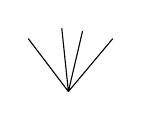
\begin{tikzpicture}[scale=.6]\draw (0,0)--(-.85,1.12) (0,0)--(-.14,1.34) (0,0)--(.3,1.28) (0,0)--(.94,1.12);\end{tikzpicture}}

\diagram{\begin{tikzcd}[ampersand replacement=\&,row sep=tiny,column sep=tiny]
\&\unsure{\omega|s}\&\&\unsure{\bar s|s'|\bar 3}\arrow[ll]\\
\&\bullet\&\unsure{s}\arrow[l]\&\bullet\arrow[l]\\
\unsure{\bar s|s|-a}\arrow[ur]\&\deleted{\unsure{s}}\arrow[u]\&\unsure{\bar s|s'|\bar 3}\arrow[u]\&s\arrow[u]\arrow[uu]\\
\&\underset{\unsure{a|x|\bullet}}{\bullet}\arrow[ul]\arrow[u]\arrow[ur]\arrow[urr]\&\&
\end{tikzcd}}

On trouve aussi que \unsure{tte|les} arête est incidente à une face (\unsure{sinon} on aurait ds $|\mathcal X|$ des pts au voisinage desquels $|\mathcal X|$ est de dim $1$ !) et \deleted{\unsure{on trouve que}}\inserted{on en conclut} que \uline{tte} \uline{arête} a \unsure{exact\textsuperscript{t}} 2 sommets\ldots

\figure{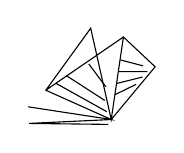
\begin{tikzpicture}[scale=.62]
\draw (0,0)--(-1.34,.6)--(-.42,1.87)--(0,0)--(.25,1.69)--(.9,1.08)--(0,0)
(-1.34,.6)--(.25,1.69) (-1.34,.6)--(0,0)--(-1.7,.26) (0,0)--(-1.68,-.08)--(-.06,-.1);
\draw (-1.13,.74)--(-.09,.16) (-.92,.9)--(-.13,.39) (-.46,1.14)--(-.11,.67)
(.08,.51)--(.51,.72) (.12,.74)--(.64,.87) (.16,.98)--(.74,.98) (.19,1.22)--(.65,1.1);
\end{tikzpicture}}
}

en faisant opérer $\sigma_{n-1},\ldots,\sigma_{p+1}$ trivialement sur $R_p$ \quad ($n\unsure{>|{\ge}}p\ge0$)

\figure{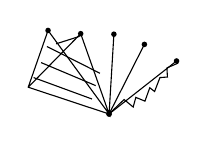
\begin{tikzpicture}[scale=.68]
\draw (0,0)--(-1.51,.5)--(-1.14,1.56)--(0,0)--(-.53,1.5)--(-1.51,.5)
(0,0)--(.09,1.49) (0,0)--(.66,1.3) (0,0)--(1.26,.99);
\draw (-1.41,.68)--(-.32,.28) (-1.27,.96)--(-.25,.53) (-1.16,1.26)--(-.17,.76) (-.99,1.31)--(-.55,1.45);
\draw (0,0)--(.28,.27)--(.45,.13)--(.5,.31)--(.67,.24)--(.76,.49)--(.85,.42)--(.95,.68)--(1.09,.69)--(1.08,.86)--(1.29,.95);
\fill (0,0) circle (.055) (-1.14,1.56) circle (.052) (-.53,1.5) circle (.052) (.09,1.49) circle (.052) (.66,1.3) circle (.052) (1.26,.99) circle (.052);
\end{tikzpicture}}

% archive sheet number: 40
